In this section we investigate the performance of our method quantitatively on the public Oxford Radar RobotCar Dataset~\cite{RadarRobotCarDatasetICRA2020}, in an urban environment, and qualitatively on two data sets that we collected in non-urban environments (\textit{Kvarntorp mine} and \textit{Volvo test track}), to demonstrate how the method generalises without site and sensor specific parameter tuning. All experiments were carried out on an i7-7700HQ 2.80~GHz laptop CPU, running in a single thread.





\subsection{Parameters}
\label{ssec:Parameters}
The full set of parameters can be seen in Table~\ref{tab:Parameter}. We tuned the parameters to an urban environment using the sequence \textit{16-13-42} in the Oxford dataset. This sequence is not included in the evaluation set, with the intention to avoid fitting parameters to the specific traffic conditions in one of the evaluated sequences. After the parameter tuning, the exact same parameters were used through all experiments, despite widely different environments and although different radar models with different range resolutions were used.

A brief evaluation of the most important parameters (performed on the Oxford dataset) can be seen in Fig.~\ref{fig:parameter_eval}. 
The results in Fig.~\ref{fig:keyframe_eval} show that the accuracy can be improved by increasing $s$ (submap keyframes) at the expense of runtime performance. 
Fig.~\ref{fig:k_eval} shows the effect of varying the number $k$ of returns in our filtering method.
Using too few ($k<12$) or too many ($k>35$) points negatively impact accuracy, but within the wide range $12\leq k \leq 35$ the method is largely insensitive to $k$.

 \begin{figure}
 \vspace{0.3cm}
  \begin{center}
    \subfloat[
    Increasing the amount of key-frames $s$
reduces the translation error but requires additional processing time. Resample factor is set to $f=3$. ]{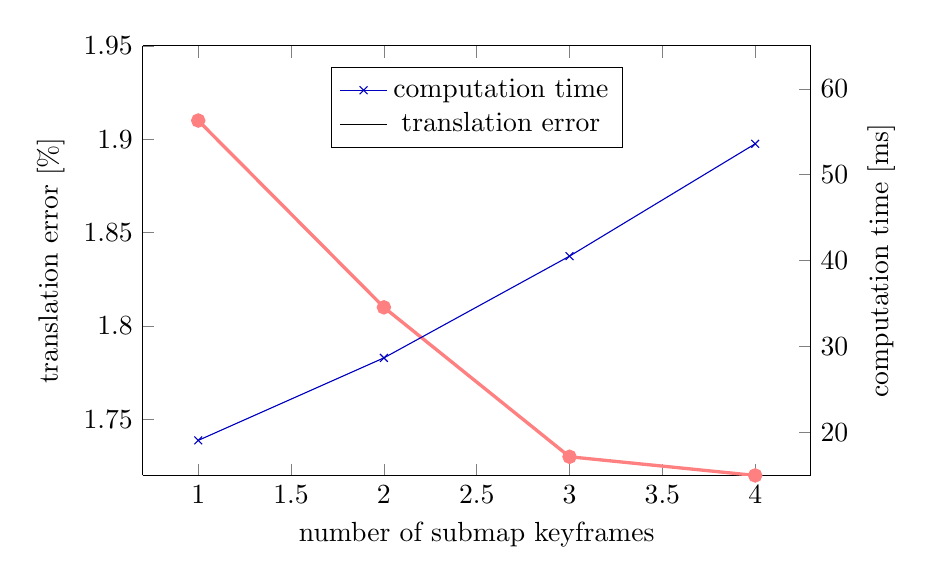
\begin{tikzpicture}

\pgfplotsset{width=7.5cm,compat=1.12}
  \pgfplotsset{
      scale only axis,
  }

  \begin{axis}[
	width   = 0.7\columnwidth,
	height  = 0.45\columnwidth,  
	ymin		= 1.72,
	ymax		= 1.95,
	legend style={at={(0.5,0.95)},anchor= north},
    axis y line*=left,
    xlabel={number of submap keyframes},
    ylabel={translation error [$\%$]},
  ]
    \addplot[mark=*,white!50!red,very thick]
      coordinates{
    (1.0000, 1.9100)
    (2.0000, 1.8100)
    (3.0000, 1.7300)
    (4.0000, 1.7200)
}; \label{plot_1_y1}

    \end{axis}

    \begin{axis}[
		width   = 0.7\columnwidth,
		height  = 0.45\columnwidth,
	ymin		= 15,
	ymax		= 65,
	legend style={at={(0.5,0.95)},anchor= north},
    axis y line*=right,
    axis x line=none,
    ylabel={computation time [ms]},
    ]

    \addplot[mark=x,blue!75!black,thin]
      coordinates{
    (1, 19.0795)
    (2, 28.6807)
    (3, 40.5221)
    (4, 53.5934)
}; \label{plot_1_y2}
    
    \addlegendimage{/pgfplots/refstyle=plot_1_y1}\addlegendentry{computation time}
    \addlegendimage{/pgfplots/refstyle=plot_1_y2}\addlegendentry{translation error}
  \end{axis}

\end{tikzpicture} \label{fig:keyframe_eval}}\hfill
    \subfloat[Within a wide range of values of \textit{k}, \ac{TITLE}  is insensitive to the exact value of \textit{k}.
A too small or too large value, however, reduces translation and rotation accuracy. ]{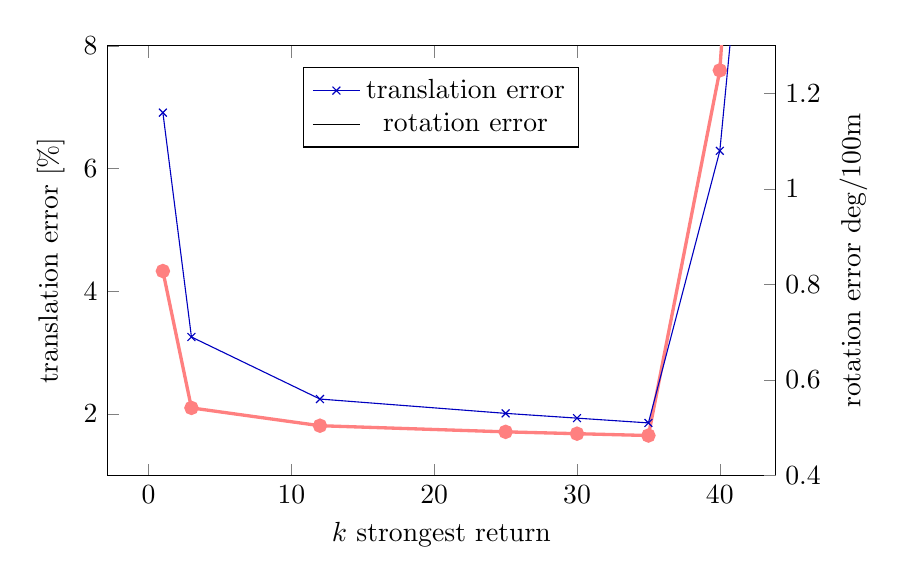
\begin{tikzpicture}
\pgfplotsset{width=7.5cm,compat=1.12}
  \pgfplotsset{
      scale only axis,
  }

  \begin{axis}[
  	width   = 0.7\columnwidth,
	height  = 0.45\columnwidth,
	ymin		= 1,
	ymax		= 8,
	legend style={at={(0.5,0.95)},anchor= north},
    axis y line*=left,
    xlabel={$k$ strongest return},
    ylabel={translation error [$\%$]},
  ]
    \addplot[mark=*,white!50!red,very thick]
      coordinates{
    (1.0000,    4.3300)
    (3.0000,    2.1000)
    (12.0000,    1.8100)
    (25.0000,   1.7100)
    (30.0000,    1.6800)
    (35.0000,   1.6500)
    (40.0000,    7.6000)
    (50.0000,   41.6100)
}; \label{plot_1_y1}

    \end{axis}

    \begin{axis}[
	width   = 0.7\columnwidth,
	height  = 0.45\columnwidth,
	ymin		= 0.4,
	ymax		= 1.3,
	legend style={at={(0.5,0.95)},anchor= north},
    axis y line*=right,
    axis x line=none,
    ylabel={rotation error $\deg$/100m},
    ]

    \addplot[mark=x,blue!75!black,thin]
      coordinates{
    (1.0000,  1.1600)
    (3.0000,  0.6900)
    (12.0000, 0.5600)
    (25.0000, 0.5300)
    (30.0000, 0.5200)
    (35.0000, 0.5100)
    (40.0000, 1.0800)
    (50.0000, 4.1900)
        
}; \label{plot_1_y2}
    
    \addlegendimage{/pgfplots/refstyle=plot_1_y1}\addlegendentry{translation error}
    \addlegendimage{/pgfplots/refstyle=plot_1_y2}\addlegendentry{rotation error}
  \end{axis}

\end{tikzpicture}     \label{fig:k_eval}}\hfill
    \caption{Accuracy/computation time using different parameters.}\label{fig:parameter_eval}
  \end{center}
  \vspace{-0.3cm}
\end{figure}



\begin{table}
\centering
\begin{tabular}{l|lll}
\\
Parameters & Value          \\    \hline
$k$                              & $12$ \\ Resample factor $f$                     & $1$ \\  $\zmin$                               & $55$ \\  Resolution $r$                          & $3.5$ \\  $\theta_\mathrm{max}$                          & $30$ \\    Huber loss    $\mathcal{L}_\delta$      & $0.1$ \\    Key-frame (dist[m]/rot[deg])            & $1.5/5^\circ$ \\  $s$                        & $3$ \\   min. sensor distance [m]                 & $5$ \\     max. sensor distance [m]                & $100$ \\   \end{tabular}
\caption{Full list of parameters. These are used for all datasets and sensors, except when explicitly mentioned in Sec.~\ref{sec:volvo_eval}. }\label{tab:Parameter}
\end{table}


\subsection{Quantitative evaluation in urban environment}
\label{sec:quantitative_eval_sec}
We provide a quantitative evaluation of the odometry accuracy and performance in a large-scale environment with ground truth positioning. The odometry accuracy was measured as proposed in the KITTI odometry benchmark~\cite{Geiger2012CVPR} using the tool~\cite{zhan2019dfvo} that computes the average translation error ($\%$) and rotation error (deg/m) over all sub sequences between $\{100,200, \ldots, 800\}$~m.

We used the public Oxford Radar RobotCar Dataset which was collected with a roof-mounted Navtech CTS350-X \ac{FMCW} radar running at $4$~Hz, configured with a range resolution of $\gamma=4.38$~cm. The dataset contains 32 traversals through a $10$-km urban environment in varied weather, lighting and traffic conditions.

In order to compare our results, we selected the same sequences that were used in the evaluation by Hong~\cite{hong2020radarslam}, both for quantitative evaluation as presented in Tab.~\ref{tab:results} and the visualization in Fig.~\ref{fig:sequences_oxford}. Learning-based methods are compared using their SCV (Spatial Cross Validation). With SCV, test and training datasets are taken from different parts of the environment, rather than selecting the training data from different traverses in the same locations. Without SCV, test and training datasets are not independent since test and training points may be neighbors~\cite{lovelace_geocomputation_2019}.



As can be seen in Tab.~\ref{tab:results}, \ac{TITLE} produces the lowest per-sequence and mean SCV error with a translation and rotation error of $1.76\%$ and $0.5$~deg/100m, followed by Barnes Dual Cart~\cite{barnes_masking_2020} ($2.78$\%), Hong odometry~\cite{hong2020radarslam} ($3.11$\%), and Cen ~\cite{8460687} ($3.72$\%).
\textit{Barnes Dual Cart}~\cite{barnes_masking_2020} achieves greater mean accuracy ($1.16$\% error) but only when training and evaluating on the same spatial location. When the authors evaluated their methods on places not seen in the training set, the error increased to from $1.76\%$ to $2.78$\%.
\ac{TITLE} provides a $14$\% lower mean odometry error compared to ~\cite{barnes_under_2020} without SCV. The method does not report SCV error in the original publication and it is unclear how well the method generalizes to new nearby locations or environments. 

We therefore argue that \ac{TITLE} method improves state-of-the-art accuracy for sparse methods, but also improves state-of-the-art among all radar odometry methods conditioned on that the evaluation is not biased with spatially overlapping training and evaluation data.


 \begin{figure}
  \vspace{0.2cm}
  \begin{center}
\includegraphics[width=0.89\hsize,trim={0cm 0cm 0cm 0cm},clip,angle=270]{figures/Oxford/Examples/highlight_start_lowres.jpg}\caption{\label{fig:oxford_overview}Incremental radar odometry using the proposed method over a $10$~km sequence from the Oxford dataset. The first and final pose estimate is highlighted and gives an indication of the total aggregated drift. }
  \end{center}
 \vspace{-0.6cm}
\end{figure}



\begin{figure*}[]
  \begin{center}
    \subfloat[10-12-32]{\includegraphics[trim={0.0cm 0cm 0cm 0cm},clip,width=0.32\hsize]{figures/Oxford/Trajectories/10-12-32.png}\label{fig:10-12-32}}\hfill
    \subfloat[16-13-09]{\includegraphics[trim={0.0cm 0cm 0cm 0cm},clip,width=0.32\hsize]{figures/Oxford/Trajectories/16-13-09.png}\label{fig:16-13-09}}\hfill
    \subfloat[17-13-26]{\includegraphics[trim={0.0cm 0cm 0cm 0cm},clip,width=0.32\hsize]{figures/Oxford/Trajectories/17-13-26.png}\label{fig:17-13-26}}\\\
    \vspace{-0.2cm}
     \subfloat[18-14-14]{\includegraphics[trim={0.0cm 0cm 0cm 0cm},clip,width=0.32\hsize]{figures/Oxford/Trajectories/18-14-14.png}\label{fig:18-14-14}}\hfill
    \subfloat[18-15-20]{\includegraphics[trim={0.0cm 0cm 0cm 0cm},clip,width=0.32\hsize]{figures/Oxford/Trajectories/18-15-20.png}\label{fig:18-15-20}}\hfill
    \subfloat[16-11-53]{\includegraphics[trim={0.0cm 0cm 0cm 0cm},clip,width=0.32\hsize]{figures/Oxford/Trajectories/16-11-53.png}\label{fig:16-11-53}}
    \caption{Evaluated Oxford sequences using \ac{TITLE}. For qualitative comparison to other methods we refer to ~\cite{hong2020radarslam}.}\label{fig:sequences_oxford}
  \end{center}
  \vspace{-0.3cm}
\end{figure*}


\begin{table*}
\centering
  \begin{adjustbox}{width=\textwidth}

\begin{tabular}{l|ll|lllllllll|l|l}
              & & & \multicolumn{1}{l}{\textbf{Sequence}}    &                                                                        \\
\textbf{Method} & \textbf{Evaluation} & \textbf{resolution}        & 10-12-32 & 16-13-09 & 17-13-26 & 18-14-14 & 18-15-20 & 10-11-46 & 16-11-53 & 18-14-46 & Mean  & \textbf{Mean SCV} & runtime (ms)   \\
\hline \\
Visual Odometry  ~\cite{Churchill2012ExperienceBN} & ~\cite{barnes_masking_2020} & N/A   & N/A        & N/A        & N/A        & N/A        & N/A        & N/A        & N/A        & N/A        &    $3.78/0.01$ & N/A   &      \\
\hline \\
SuMa (Lidar)~\cite{behley2018rss}  & ~\cite{hong2020radarslam }& N/A  & $1.1/0.3$ & $1.2$/$0.4$ & $1.1/0.3$ & $0.9/0.1$ & $1.0/0.2$  & $1.1/0.3$        & $0.9/0.3$        & $1.0/0.1$        & $1.16/0.3$    & $1.03/0.3$  &       \\
\hline \\
Cen~\cite{8460687}    &   ~\cite{barnes_masking_2020} & $0.175$& N/A        & N/A        & N/A        & N/A        & N/A        & N/A        & N/A        & N/A        & $3.72/0.95$    & $3.63/0.96$ &        \\
Robust Keypoints~\cite{barnes_under_2020}    &  & $0.346$    & N/A        & N/A        & N/A        & N/A        & N/A        & N/A        & N/A        & N/A        & $2.05/0.67^*$    & N/A  &         \\
Barnes Dual Cart~\cite{barnes_masking_2020} & & $0.043$ & N/A        & N/A        & N/A        & N/A        & N/A        & N/A        & N/A        & N/A        & $\bm{1.16/0.3}^*$    &   $2.784/0.85 $ &\\
Hong odometry~\cite{hong2020radarslam} & &$0.043$ & $2.98/0.8$        & $3.12/0.9$        & $2.92/0.8$        & $3.18/0.9$        & $2.85/0.9$        & $3.26/0.9$        & $3.28/0.9$        & $3.33/1$        & $3.11/0.9$    & $3.11/0.9$ &        \\
\ac{TITLE} (ours) &  & $0.043$ & \textbf{1.64/0.48}          & \textbf{1.86/0.52}        & \textbf{1.66/0.48}        & \textbf{1.71/0.49}        & \textbf{1.75/0.51}        & \textbf{1.65/0.48}        & \textbf{1.99/0.53}        & \textbf{1.79/0.5}        & 
1.76.0.50    & 
$\bm{1.76\pm0.12/0.50\pm0.02}$  & $18\pm 0.4$ 
\end{tabular}
  \end{adjustbox}

\caption{Evaluation on 8 sequences with different methods and sensor modalities on the Oxford Radar RobotCar dataset~\cite{RadarRobotCarDatasetICRA2020}.  Results are given in (\% translation error / deg/$100$~m). Note the difference between columns "Mean" and "Mean SCV". In "Mean" column, methods marked $^*$ cannot be compared directly as these are trained and evaluated on the same spatial location. The most relevant number for comparison is instead "Mean SCV" which ensures that test and training data are not correlated by using spatial cross validation. 
}
\label{tab:results}
\vspace{-0.2cm}
\end{table*}












\subsection{Qualitative evaluation}
In order to assess the generality of the method, additional non-urban  data was collected. We perform a qualitative evaluation of radar odometry in two different industrial scenarios using 
another Navtech \ac{FMCW} radar model,
CIR154XH. 
For these datasets, the sensor was configured with range resolution $\gamma=17.5$cm, with $400$ azimuth bins. Ground truth positioning is missing in these datasets. However, we estimate the error between the first and final scan by comparing the offset between duplicated landmarks in the map which gives a rough indication of odometry drift.


\subsubsection{Evaluation in semi-structured outdoor environment -- Volvo CE}
\label{sec:volvo_eval}

The first dataset was collected from a test track for wheel loaders and dump trucks in a partly forest environment driven at an approximate speed of $10$km/h. The track consists mainly of gravel roads at various slopes and the radar sensor was mounted on the driver cabin of a Volvo wheel loader (see Fig.~\ref{fig:volvo_test_track_and_vehicle}). The larger loop in Fig.~\ref{fig:volvo_test_track_and_vehicle} is $1150$ meters long. After completing the larger gravel-road loop, two smaller loops were traversed on uneven paths inside the forest reaching a total trajectory length of $1605$ meters. We expect this highly cluttered environment to be challenging for \ac{TITLE} that attempts to reconstruct and utilize surface normals.








The estimated odometry and a corresponding map, obtained without changing parameters from the urban dataset, is depicted in Fig.~\ref{fig:volvo_oxford_parameters}. The maximum translation error is $15$~m ($1.3$\%) over the large loop. We notice that $\zmin=55$ is too low in combination with the sensor model and cluttered forest environment, however, \textit{k-strongest filtering} limits the amount of noise included in the filtered point cloud. We also note that motion compensation can have a negative impact in this dataset. For that reason, we made an attempt to improve the odometry by increasing the power threshold $\zmin=85$, by switching off motion compensation, and by increasing surface point density to $f=3$. These parameters reduced the estimated error to $2.5$~m ($0.2)$\% as depicted in Fig.~\ref{fig:volvo_full_submap}. For comparison, we plot the odometry with updated parameters but with a single submap keyframe $s=1$, this increases the error to $5~$m ($0.4$\%) as seen in Fig.~\ref{fig:volvo_full_nosubmap}.
In line with our previous results, increasing the number of submap keyframes reduces the drift. This can be seen by the relative increase in map blur in Fig.~\ref{fig:volvo_full_nosubmap} ($s = 1$) compared to Fig.~\ref{fig:volvo_full_submap} ($s = 3$). We believe this is because additionally constraining the registration reduces pose estimate noise and increases robustness due to uneven driving conditions, especially in the forest.



 \begin{figure} 
 \vspace{0.2cm}
  \begin{center}
    \subfloat[Vehicle test track. A wheel loader with radar starts inside the white tent (right) and is driven in a large loop on a gravel road and then in two smaller loops on an uneven path in the forest. The full driven trajectory (seen in red) is imported from Fig.~\ref{fig:volvo_full_submap}.
    The locations of the photos in figure (b) and (c) are indicated along the trajectory.
    ]{\begin{tikzpicture}
    \node[anchor=south west,inner sep=0] at (0,0) {\includegraphics[trim={0.0cm 0cm 0cm 0.2cm},clip,width=0.99\hsize]{figures/Volvo/overlayed_eskilstuna_downsampeld.jpg}};
    \node[white!70!white] at(1.6,5.7) {(\textbf{b})};
    \node[white!70!white] at(3.5,5.3) {(\textbf{c})};
    \end{tikzpicture}}
\\
        \subfloat[Driving on a narrow uneven path in the forest. ]{\includegraphics[trim={0.0cm 0cm 0cm 0cm},clip,height=43mm]{figures/Volvo/loader_forest_downsampled.jpg}\label{fig:volvo_forest}}\hfill
        \subfloat[Driving on a gravel road uphill.]{\includegraphics[trim={0.0cm 0cm 0cm 0cm},clip,height=43mm]{figures/Volvo/loader_road_downsampled.jpg}\label{fig:volvo_road}}\hfill \\
    
    \caption{Overview of semi-structured VolvoCE dataset.\label{fig:volvo_test_track_and_vehicle}}
  \end{center}
  \vspace{-0.8cm}
  \end{figure} \begin{figure}
\vspace{0.2cm}
  \begin{center}
    \subfloat[Full estimated trajectory (red) and map (black), obtained reusing parameters tuned for the Oxford urban dataset. The maximum estimated large loop error is $15$~m ($1.3$\%). Grid size ($10\times 10$)~m.  ]{\includegraphics[trim={0.0cm 0cm 0cm 0cm},clip,width=0.89\hsize]{figures/Volvo/same_parameters.png}\label{fig:volvo_oxford_parameters}}\hfill 
    \\
    \subfloat[Odometry improved by tailoring parameters to the VolvoCE dataset (motion compensation switched off, $\zmin=85$, $f=3$). The Map is blurred around revisited regions of the large loop due to odometry drift but fairly sharp around the small loop. We estimate the maximum large loop position error to be $2.5$~m ($0.2\%$).]{\includegraphics[trim={0.0cm 0cm 0cm 0cm},clip,width=0.89\hsize]{figures/Volvo/5.png}\label{fig:volvo_full_submap}}\hfill \\
    \subfloat[Full estimated trajectory with a single key-frame. The maximum large loop error is estimated to be $5$~m ($0.4\%$ error). The map around the large and small loop is more distorted compared to \ref{fig:volvo_full_submap}.]{\includegraphics[trim={0.0cm 0cm 0cm 0cm},clip,width=0.89\hsize]{figures/Volvo/nosubmap/no_submap_full.png}\label{fig:volvo_full_nosubmap}}\hfill \\
    \caption{Qualitative evaluation in VolvoCE dataset using various parameters.\label{fig:volvo_after_revisit}}
  \end{center}
  \vspace{-0.5cm}
\end{figure}



\subsubsection{Evaluation in mine -- Kvarntorp}
\label{sec:kvarntorp_eval}
In another experiment we mounted the Navtech CIR154XH radar on a car and drove through a $1235$-m long loop in an underground mine, at an approximate speed of $10$~km/h. The environment is depicted in Fig.~\ref{fig:kvarntorp_example}. The solid walls are highly radar-reflective and the interaction between radar, mountain walls and the car gives rise to a large amount of strong multi-path reflections. In contrast to the other evaluated datasets, the tunnels in parts of this environment have limited features that can constrain the registration in the longitudinal direction. 

Reusing the parameters tuned for Oxford dataset, we found that our method was able to reconstruct an accurate map of the environment with an estimated final position error of $15$~m ($1.2)$\% translation error. There are no visible errors in the passages between the top and bottom aisles in Fig.~\ref{fig:kvarntorp_example}, which is an indication that the method works well, even in a feature poor environment.




%
